\chapter{Modèle d'architecture CxSOM}
\graphicspath{{02-SOM/}}
\minitoc

Nous proposons dans cette thèse un modèle d'architecture de cartes auto-organisatrices, CxSOM. Par ce modèle, on associe des cartes auto-organisatrices en architecture afin de réaliser des tâches de mémoire associative: apprendre un modèle de relation entre des ensemble de données issues de plusieurs modalités. 
On souhaite que ce modèle soit générique, permette de construire n'importe quel forme et taille d'architecture, et aie la possibilité d'intégrer des connexions récurrentes. Notre démarche est d'abord de proposer un nouveau modèle de calcul général à base de cartes auto-organisatrices; des applications plus spécifiques pourront être développées à partir de cette méthode.


On définit une \emph{architecture} de carte un réseau composé de plusieurs modules qui sont chacun des cartes de Kohonen, dans lequel des connexions sont définies entre ces éléments. Ces connexions ont un sens: on parle d'une connexions d'une carte A vers une carte B. Le but de ces connexions est de coupler l'apprentissage de plusieurs cartes. 
Dans une architecture, on peut construire un graphe $G$ orienté, dont les noeuds sont des cartes. La connexion d'une carte A vers une carte B est indiquée par la présence d'une arête de A vers B. On appelle architecture \emph{non-hiérarchique} une architecture pour laquelle $G$ n'est pas un arbre: il présente des boucles. Un exemple d'architecture non-hiérarchique est par exemple représenté en figure~\ref{fig:archi_non_hierarchique}. Certaines cartes sont connectées dans les deux sens, d'autres en boucle. Ces architectures non-hiéarchiques seront utilisées pour des tâches de mémoire associative: Chaque carte de l'architecture apprend sur des entrées, $A,B,C,D,E$ dans la figure, liées par un modèle. Les cartes cherchent chacune à apprendre leurs entrées, et l'architecture dans sa globalité est là pour apprendre les relations existant entre les données. 

Dans ce chapitre, nous détaillons le modèle CxSOM développé et étudié durant cette thèse, permettant de construire des architectures non-hiérarchiques de cartes auto-organisatrices. Nous présentons en premier lieu le formalisme d'une carte de Kohonen classique, dont sont dérivées les cartes auto-organisatrices utilisées dans les architectures CxSOM. Nous expliquerons ensuite les choix de développement sur lesquels nous nous sommes appuyés pour développer le modèle; enfin, le modèle sera présenté sur un exemple d'architecture à deux cartes et illustré, puis nous le formaliserons pour le cas général de $n$ cartes connectées dans une architecture. Le glossaire des notations est retrouvable en Annexe.

\begin{figure}
\centering
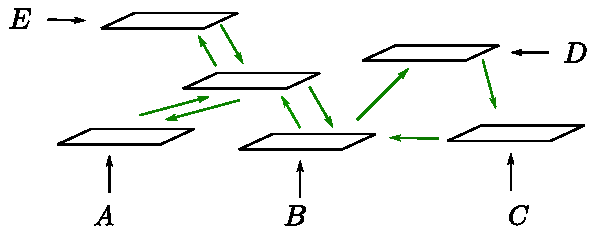
\includegraphics[width=0.6\textwidth]{architecture.pdf}
\caption{Exemple d'architecture modulaire \emph{non-hiérarchique} de cartes de Kohonen. Les entrées sont $A,B,C,D,E$ quelconques. Chaque carte peut ou non prendre une entrée ; les connexions sont réciproques ou non.}
\label{fig:archi_non_hierarchique}
\end{figure}


\section{Carte de Kohonen classique}\label{sec:kohonen}
Chaque carte de Kohonen intervenant dans l'architecture CxSOM est directement dérivée de l'algorithme d'une carte de Kohonen classique \cite{Kohonen1982}. Le principe général d'une carte de Kohonen a été décrit dans le chapitre précédent; nous définissons ici plus précisément le modèle et les équations qui serviront de base pour la définition de l'algorithme CxSOM.

\subsection{Algorithme et notations}
Une carte de Kohonen est un graphe, généralement une ligne 1D ou une grille 2D de $N$ noeuds. Nous utiliserons dans cette thèse des cartes en une et deux dimensions, c'est à dire des lignes et des grilles. Les notations et le modèle présentés ici sont toutefois applicables à des cartes de dimension et topologies quelconques.

L'algorithme et les notations sont résumés en figure~\ref{fig:one_map_not}. Une carte de Kohonen apprend sur des entrées, notées $\inpx_t$, tirées dans un espace d'entrée $\mathcal{D}$. A chaque noeud de la carte est associé un poids, appelé aussi prototype, noté $\w_e \in D$. Sa \emph{position} dans la carte est indexée par $p$. Nous choisissons d'indexer les positions entre $0$ et $1$. L'ensemble des poids est noté ${\w_e(p), p \in [0,1]}$.
Une étape $t$ de l'algorithme de mise à jour d'une carte de Kohonen suit les étapes suivantes:
\begin{enumerate}
\item\label{enum:inp} Une entrée $\inpx_t$ est présentée à la carte.
\item\label{enum:act} Une \emph{activité} $a_e(\inpx_t,p)$ est calculée dans la carte. La fonction d'activité choisie est une activation gaussienne:
\begin{equation}\label{eq:act1som}
a_e(\inpx_t,p) = \exp{\frac{\lVert \inpx_t-\w\ext(p) \rVert ^2}{2\sigma^2}}
\end{equation}
Cette étape est déjà une modification de l'algorithme original de Kohonen.
Dans la version classique, on calcule lors de cette étape les distances entre l'entrée et les poids $\lVert \inpx_t - \w_e(p) \rVert$, et le BMU est choisi comme l'unité dont le poids présente la plus petite distance à l'entrée. 
Ici, on prendra comme BMU l'unité ayant l'activité la plus élevée.
\item\label{enum:bmu} L'unité ayant l'activité maximale est la \emph{Best Matching Unit} de la carte. Sa position est notée $\bmu$.
\item Chaque poids $\w_e$ est déplacé vers l'entrées $\inpx$. Le déplacement est pondéré par une \emph{fonction de voisinage} $H(\bmu,p)$, dépendant de la position de chaque unité dans la carte à la best matching unit. Elle est maximale en $p = \bmu$ et décroissante autour de cette position. Dans notre étude, la fonction de voisinage est triangulaire, donc maximale en $\bmu$, décroissante sur le \emph{rayon de voisinage} $h_e$ et nulle sinon. Cela signifie que le BMU est déplacé vers l'entrée, et les poids des unités voisines du BMU dans un rayon $h_e$ sont également déplacés, mais selon un plus faible coefficient.
\begin{equation}
\w_e(p,t+1) = \w_e(p,t) + \alpha H(\bmu,p)(\inpx_t - \w_e(p,t))
\label{eq:update}
\end{equation}
\end{enumerate}


\begin{figure}
\centering
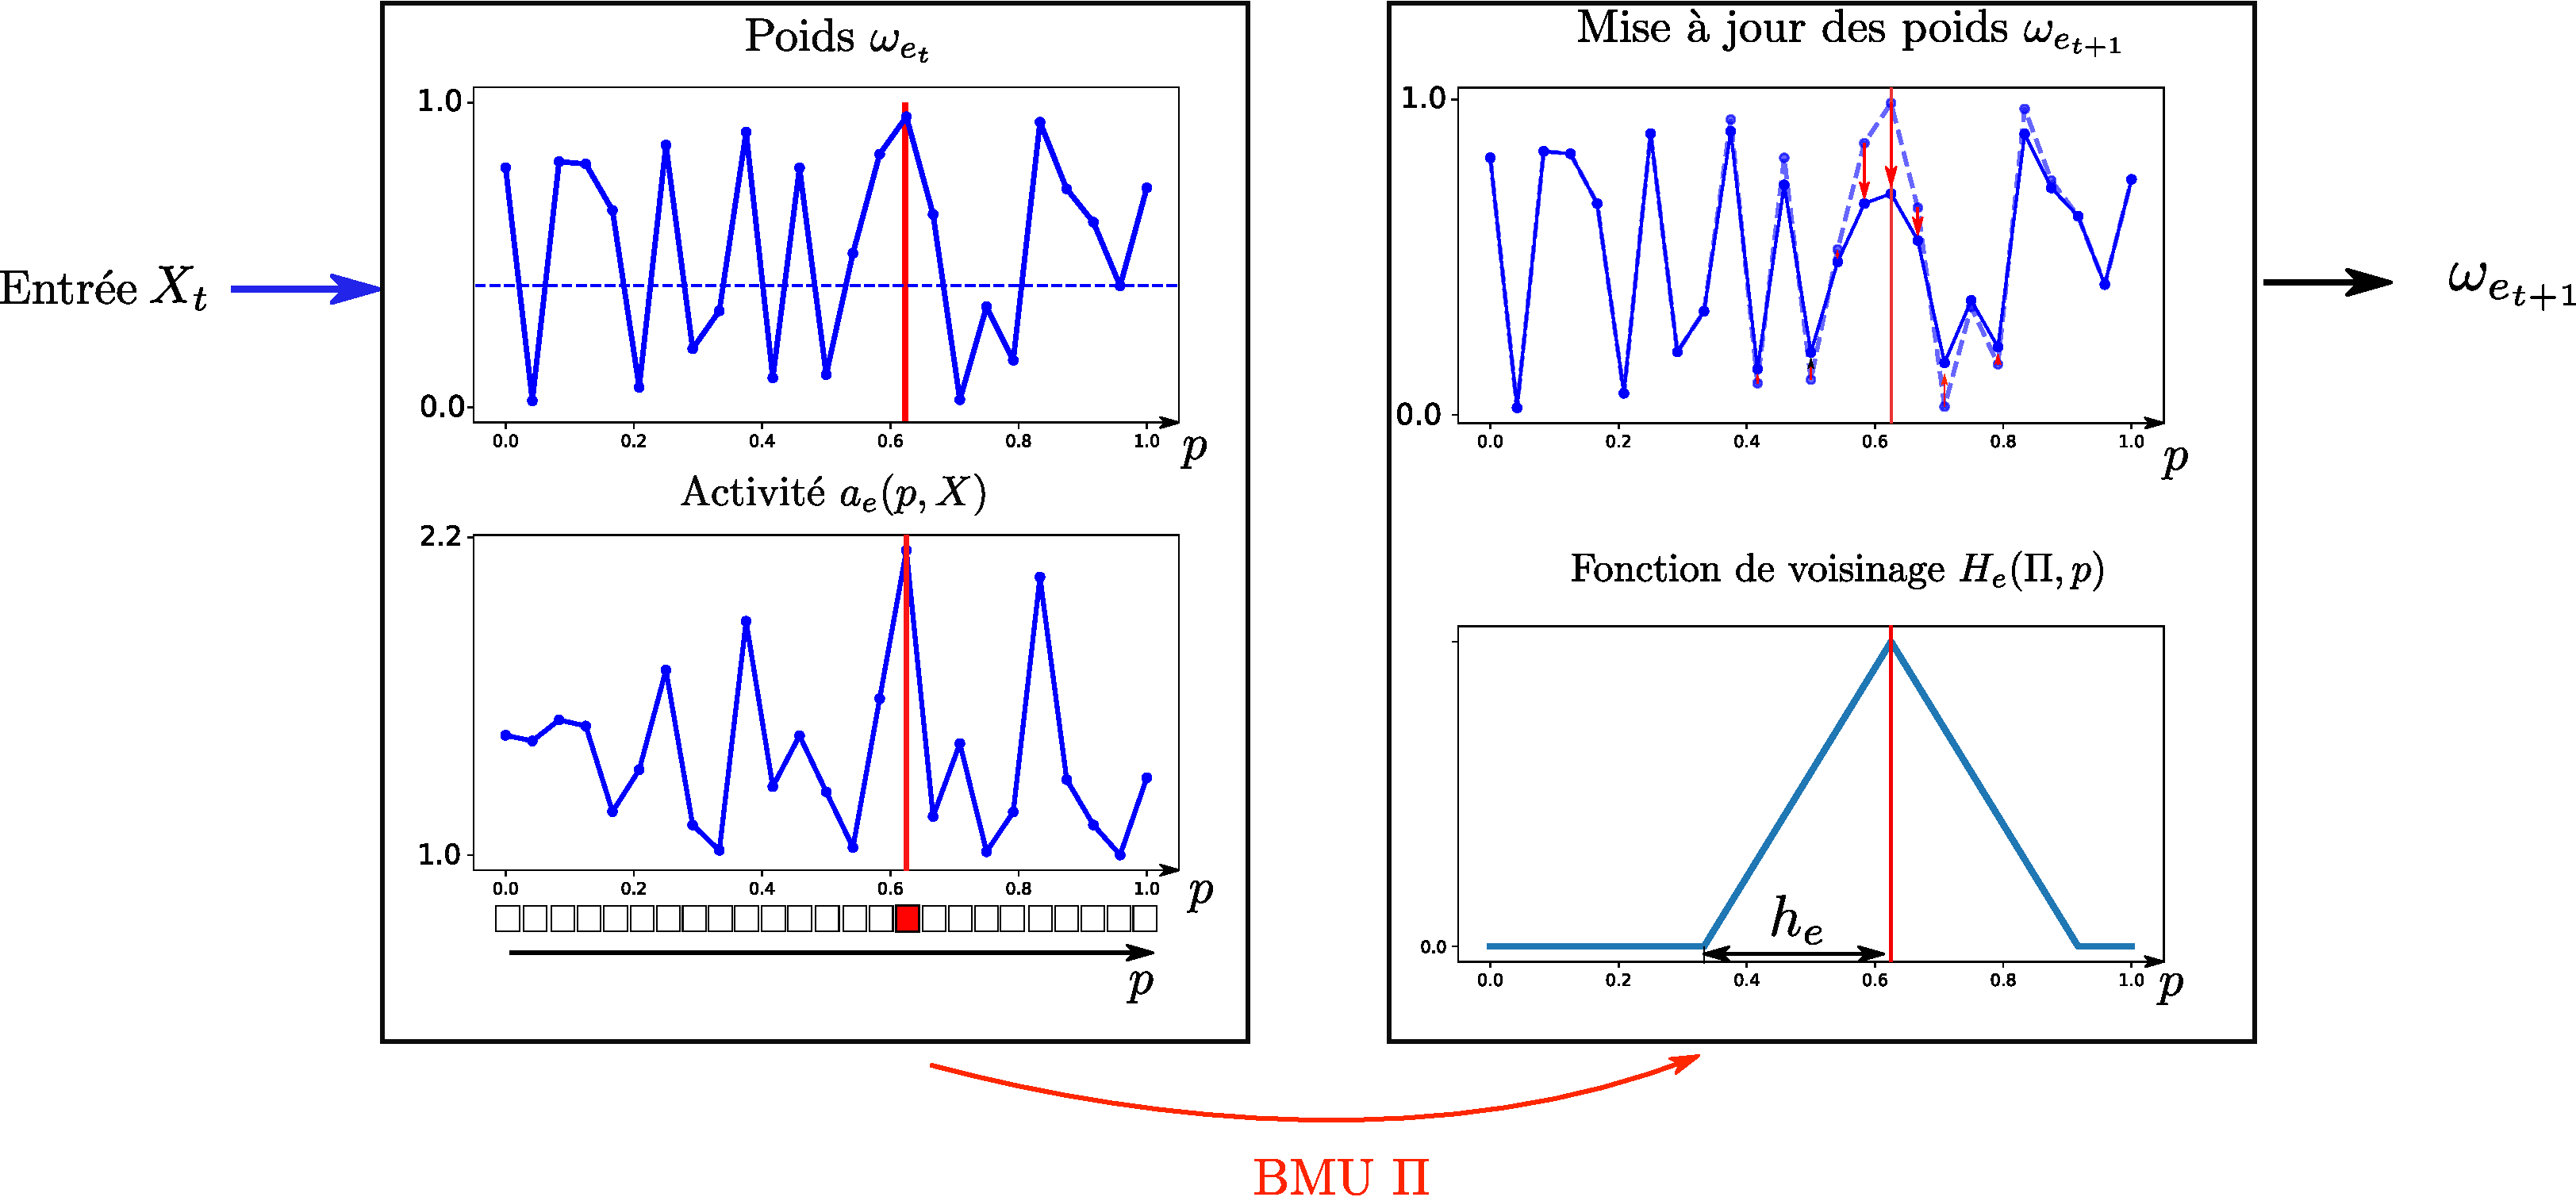
\includegraphics[width=\textwidth]{one_map_one_layer2.pdf}
\caption{Notations utilisées dans une carte de Kohonen simple. Les 4 étapes d'une itération d'apprentissage sont présentées: 1. Présentation de l'entrée, 2. Calcul de l'activité, 3. Choix du BMU, 4. Mise à jour des poids.}
\label{fig:one_map_not}
\end{figure}


\subsection{Paramètrage d'une carte de Kohonen}
La qualité d'apprentissage, appelée aussi dépliement, d'une carte de Kohonen est gérée par plusieurs paramètres. Nous détaillons ici les choix de paramètres effectués. Les paramètres supplémentaires introduits par la version CxSOM seront présentés en partie \ref{sec:params}.

\subsubsection{Taux d'apprentissage $\alpha$}
Le taux d'apprentissage $\alpha$ détermine la proportion dans laquelle chaque poids est déplacé vers l'entrée lors de sa mise à jour, selon l'équation~\ref{eq:update}. Dans l'algorithme classique, ce taux d'apprentissage décroit au cours de l'apprentissage. Au début de l'apprentissage, $\alpha$ est élevé, ce qui assure un dépliement rapide de la carte. $\alpha$ est ensuite diminué manuellement tout au long de l'apprentissage. Cette décroissance assure la convergence des poids de la carte au cours de l'apprentissage.
Dans l'algorithme CxSOM, nous utiliserons un taux d'apprentissage constant au cours de l'apprentissage. L'organisation des poids sera initialement un peu plus lente qu'une carte classique, mais cela permet de garder les paramètres constant au cours de l'apprentissage.
Nous observerons qu'en une dimension, la convergence des poids de la carte est quand même assurée.

\subsubsection{Topologie de la carte}
Le graphe supportant la carte de Kohonen peut présenter diverses formes, comme détaillé en section\ref{sec:som001}. Les notations et l'algorithme CxSOM que nous présentons dans ce chapitre sont applicables à toutes les formes de cartes. Les expériences et l'évaluation du modèle se concentrent quant à elles sur des lignes 1D et des grilles 2D, et omettent les formes de graphes quelconques. Ce choix est d'abord motivé par le fait que les lignes et les grilles étant les formats de cartes les plus courants rencontrés dans la littérature. On parle souvent de cartes 1D et cartes 2D lorsqu'on parle de cartes de Kohonen, en sous-entendant le format de ligne ou de grille du graphe support. Ces formes de cartes permettent de plus d'avoir une correspondance directe entre l'espace des positions $p \in [0,1]$ et un plan 1D ou 2D. Un exemple de dépliement d'une carte 1D sur des données 1D uniformément distribuées entre 0 et 1 est représenté en figure~\ref{fig:depliement}.


Comme évoqué au chapitre précédent, la spécificité des cartes de Kohonen tient à l'organisation des prototypes sous forme de continuum. Mais lorsqu'on parle de continuité des prototypes dans une carte de Kohonen, il s'agit en fait d'une relation de proximité et d'ordre entre des prototypes discrets: prenons $p_1$, $p_2$, $p_3$ positions dans la carte, telle que $\lVert p_1 - p_2 \rVert \leq \lVert p1 - p3 \rVert$. Alors $\lVert \w_e(p_1) - \w_e(p_2) \rVert \leq \lVert \w_e(p1) - \w_e(p_3) \rVert$. En français, \emph{si deux unités sont proches dans la carte, alors leurs prototypes sont proches dans l'espace d'entrée}. Dans une carte classique, on attend que cette relation soit vérifiée sur toute la carte pour parler de carte bien dépliée, impliquant un ordre entre données. C'est le cas par exemple à l'itération 1500 de la figure~\ref{fig:depliement}. Cependant, on peut aussi parler de continuité des poids de la carte si cette relation est seulement vérifiée localement, comme à l'itération 500 de la figure~\ref{fig:depliement}.

Le format de ligne et de grille d'une carte de Kohonen permet d'étendre cette notion de proximité entre prototype à une continuité des poids au sens mathématique, par interpolation. La carte peut alors être assimilée à une fonction:
\begin{equation*}
\begin{array}{ccccc}
M& : & [0,1]^2 \; \text{ou} \;[0,1] & \to &  \mathcal{D} \\
 & & p & \mapsto & \w_e(p) \\
\end{array}
\end{equation*}

Cette continuité est une des puissances d'une carte de Kohonen en tant qu'algorithme de quantification vectorielle. Elle permet de directement associer des éléments de l'espace d'entrée à des positions $p$ de faible dimension. Dans le modèle CxSOM, nous traitons les positions $p$ comme un ensemble continu dans lequel nous réaliserons des opérations. 


Au cours de l'apprentissage, les poids d'une carte se rapprochent de la distribution des données. On parlera de \emph{dépliement} d'une carte pour parler de son apprentissage. Un exemple de dépliement d'une carte 1D sur des données 1D est tracé en figure~\ref{fig:depliement}.
Dans ce cas, la carte 1D se rapproche de la fonction identité (ou moins l'identité): les poids sont ordonnés entre 0 et 1.
Lorsque la dimension des données est plus grande que celle de la carte, par exemple des points 2D ou des images (256 dimension), la carte formera des plis de manière à remplir l'espace $\mathcal{D}$ (voir figure~\ref{fig:som1d}, section~\ref{sec:som001} ) 

\begin{figure}
\centering
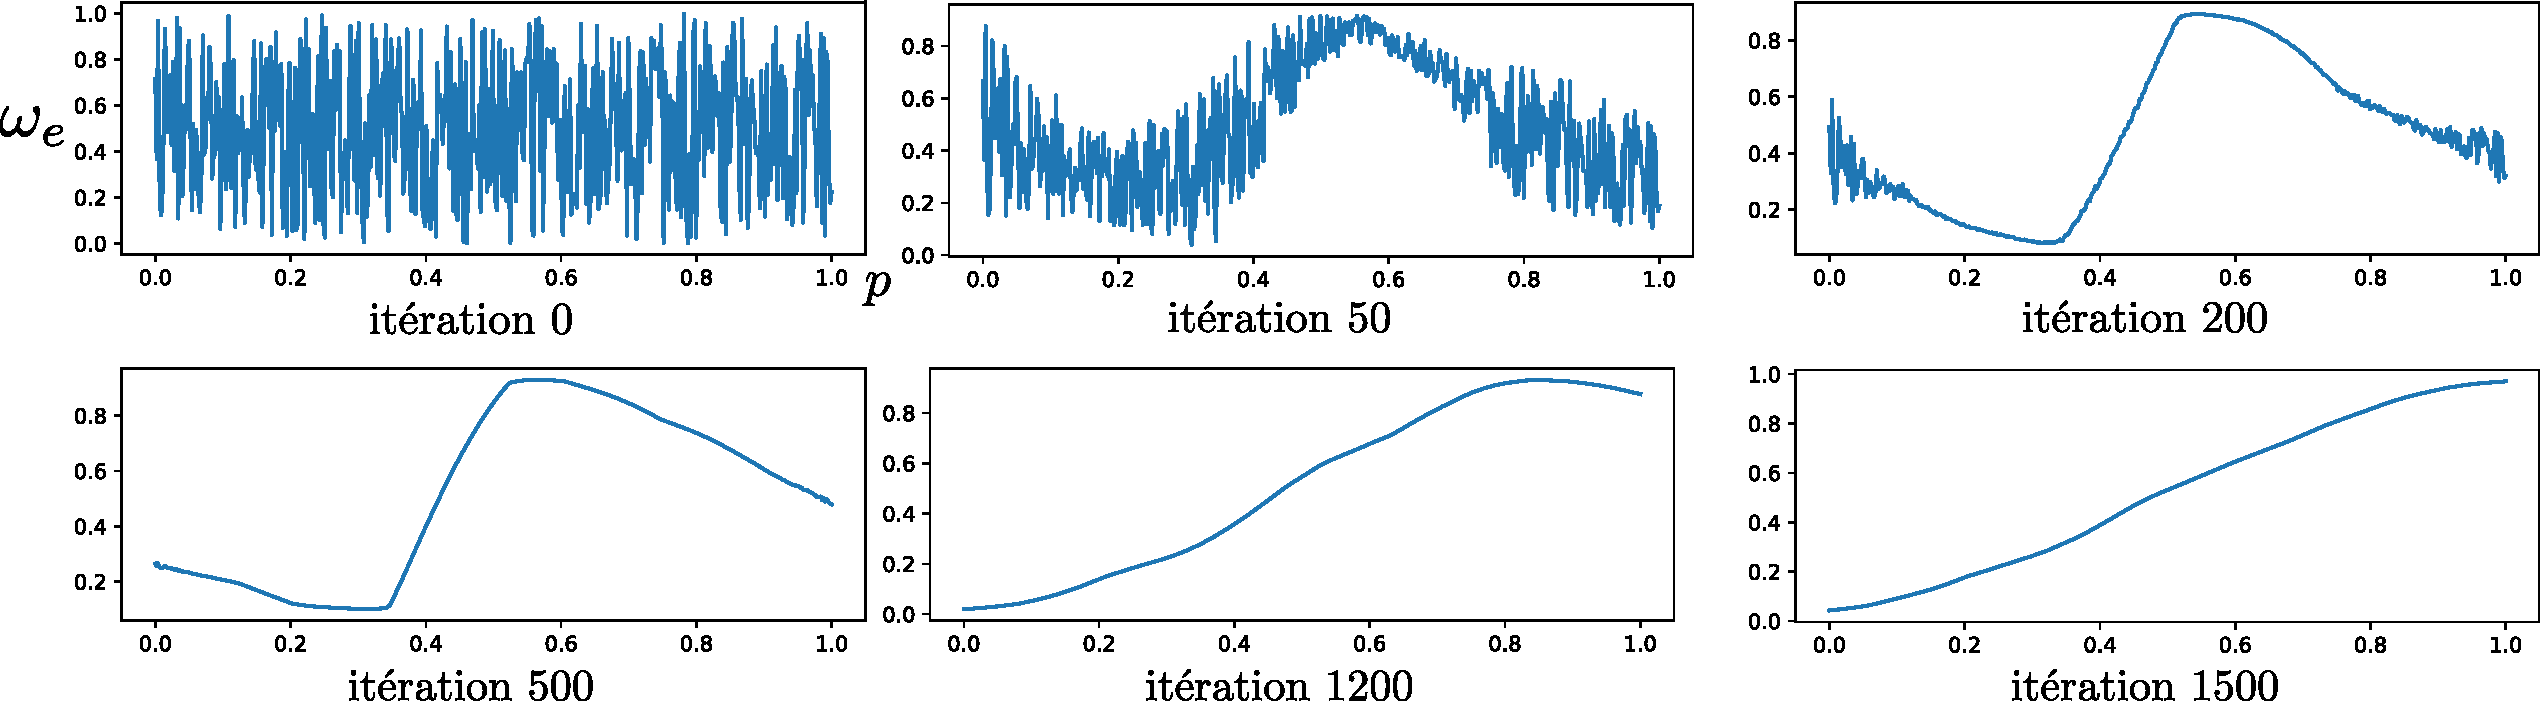
\includegraphics[width=\textwidth]{depliement_1D.pdf}
\caption{Exemple de dépliement d'une carte 1D de taille 500, sur des données 1D $\inpx \in [0,1]$. Les paramètres $h\ext = 0.2, \: \alpha = 0.2$ ont été gardé constants dans cet exemple. Une carte bien dépliée est assimilable à l'identité, comme sur cet exemple, ou moins l'identité. Ces configurations sont les deux seules pour lesquels les poids sont tous ordonnés suivant un ordre croissant ou décroissant.}
\label{fig:depliement}
\end{figure}


\subsubsection{Nombre de neurones d'une carte}
Le nombre de neurones d'une carte définit le niveau de quantification qu'on souhaite effectuer. Pour des opérations de classification, on choisira un nombre de neurones plus élevé que le nombre de classes, afin de pouvoir avoir plusieurs prototypes par classe.
Dans cette thèse, nous utilisons principalement des cartes 1D comportant 500 noeuds.

\subsubsection{Rayon de voisinage}
Le choix de la fonction de voisinage est déterminant dans la topologie de la carte, et en particulier le rayon de voisinage $h_e$.
Cette valeur détermine quelles unités voisines du BMU seront affectées par le déplacement du BMU.
Plus le rayon $h_e$ est grand, plus la partie de la carte déplacée vers l'entrée lors de la mise à jour est étendue. Un grand rayon d'apprentissage permet un dépliement plus rapide de la carte de Kohonen, mais l'apprentissage est peu précis car chaque poids est une moyenne d'un grand nombre de vecteurs. Les données déjà représentées sont rapidement oubliées par le déplacement des poids.
Un petit rayon d'apprentissage permet de déplacer les poids concentrés dans une petite région sans affecter toute la carte. Cela permet donc d'apprendre de nouvelles entrées sans oublier les parties déjà apprises. Par contre, utiliser un petit rayon de voisinage au début de l'apprentissage empêche une carte de bien se déplier et d'apprendre une structure globale des données. On doit donc trouver un compromis entre apprentissage de nouvelles données et mémoire des données déjà apprises.
Dans l'algorithme classique, ce compromis est trouvé en faisant décroitre le rayon de voisinage au cours de l'apprentissage. Un grand rayon de voisinage permet à la carte de se déplier rapidement en apprenant une structure globale des données. Sa décroissance permet d'affiner l'apprentissage des données à un niveau plus fin. 
Contrairement à la plupart des SOM classique, nous garderons des rayons de voisinage constants dans CxSOM. Ainsi, une étape de dépliement des cartes ne dépend pas de l'itération mais seulement de l'état précédent de la carte et de l'architecture.
%TODO citer des papiers recherchant un bon ensemble de paramètres pour l'algorithme de cartes auto-organisatrices.

\section{Motivations du modèle CxSOM}
A partir du modèle de carte de Kohonen détaillé en section \ref{sec:kohonen}, nous proposons une version de carte auto-organisatrice servant de bloc de base pour construire des architectures non-hiérarchique de cartes. L'idée de construire une telle architecture est de traiter plusieurs ensembles de données de façon jointe, pour réaliser de la mémoire associative.
Nous présentons tout d'abord les choix de développement effectués pour créer le modèle d'architecture.

\subsection{Champ d'application: mémoire associative}
L'architecture CxSOM a pour but de développer une mémoire \emph{associative} au sein d'une architecture de cartes. On considère donc un ensemble d'espaces $\mathcal{D}\m{1}, \cdots , \mathcal{D}\m{n}$, différentes \emph{modalités} qu'on cherche à apprendre de façon associative. Les entrées présentées à une architecture de cartes seront $(\inpx\m{1}, \cdots, \inpx\m{n}) \in \mathcal{D}\m{1} \times \cdots \times \mathcal{D}\m{n}$. Pour pouvoir développer une mémoire associative, on se place dans des cas où les modalités considérées ne sont pas indépendantes les unes des autres : les distributions marginales $\inpx\m{i}$ ne sont pas indépendantes. Lorsqu'on tire une entrée pour la présenter à une carte, on tire une entrée jointe $(\inpx\m{1}, \cdots , \inpx\m{n})$, puis chaque composante est présentée à la carte qui lui correspond. Pour respecter l'homogénéité des entrées necessaires à l'apprentissage d'une carte auto-organisatrice, on normalise les espaces $\mathcal{D}\m{i}$ pour que toutes les entrées soient à valeur dans $[0,1]^k$, $k$ la dimension de $\mathcal{D}\m{i}$.

Dans les exemples de cette thèse, on tire des entrées jointes en 3 dimensions, donc chaque composante 1D est présentée à une carte. Chaque modalité est la coordonnée sur un des axes du point 3D tiré. Nous utiliserons par exemple, en tant qu'espace dont les modalités sont dépendantes, un ensemble de points sur un cercle en une dimension dans un espace en trois dimensions. Chaque coordonnée $X$, $Y$, $Z$ dépend alors des deux autres coordonnées. On évaluera comment l'architecture que nous présentons dans cette partie apprend les données mais surtout leurs relations. 

Les exemples porteront sur des modalités en une dimension, mais les dimensions de chaque modalité peuvent être quelconque.

\begin{figure}
\centering
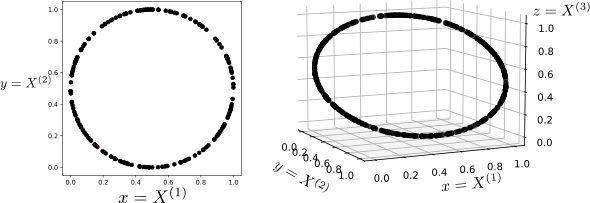
\includegraphics[width=\textwidth]{inputs_3som}
\caption{Exemple de disposition d'entrées. Les modalités associées à différentes cartes sont les coordonnées $x,y,z$ de chaque point. Dans une telle disposition, les modalités dépendent les unes des autres: développer une mémoire associative signifie apprendre le modèle de relation existant etre $x,y$ et $z$, c'est à dire le cercle.}
\label{fig:inputs}
\end{figure}

\subsection{Description de l'architecture}

Nous avons vu au chapitre précédent la notion de contexte transmise entre cartes. Dans CxSOM, on choisit de se placer dans le paradigme de transmission de la position du BMU entre cartes: on connecte une carte B à une carte A en donnant la position du BMU de B en entrée à la carte A. 
Ce paradigme de partage de positions rappelle à la fois le modèle hiérarchique HSOM~\cite{lampinen_clustering_1992}, et les modèles de cartes récurrentes s'appuyant sur SOMSD \cite{hammer_recursive_2004,hagenbuchner_self-organizing_2003,fix20}.


Contrairement aux cartes hiérarchiques HSOM dans lesquelle la position du BMU est la seule entrée d'une carte de plus haut niveau, chaque carte de l'architecture peut posséder une entrée principale propre issue d'une modalité $\inpx\m{i}$, l'entrée \emph{externe}. L'entrée ou les entrées correspondant aux positions des BMUs d'autres cartes sont considérées comme une entrées supplémentaires d'une carte. Les cartes auto-organisatrices dans le modèle CxSOM prennent donc un nombre arbitraire d'entrées, dont certaines sont les BMUs d'autres cartes. On appelle ces entrées internes à l'architecture les entrées \emph{contextuelles} d'une carte.
L'algorithme d'apprentissage d'une carte auto-organisatrice prenant une position de BMU en tant que contexte est similaire à celui d'une carte classique, comprenant:
\begin{enumerate}
\item\label{etape:entree} Présentation de son entrée à la carte 
\item\label{etape:bmu} Recherche du BMU par calcul d'activité
\item\label{etape:maj} Mise à jour des poids selon une fonction de voisinage
\end{enumerate}

Chaque carte aura maintenant plusieurs entrées: une entrée \emph{externes} dans un espace d'entrée, facultative, et $k$ entrées \emph{contextuelles} qui sont les positions des BMUs des cartes qui lui sont connectées. 
La recherche du BMU doit être modifiée par rapport à la méthode originale : les rétroactions entre les cartes sont autorisées, la position du BMU de la carte A va donc influencer la position du BMU de la carte B, lequel modifie à nouveau le BMU de la carte A, etc. 

Notre algorithme implémentera deux modifications principales par rapport à l'algorithme d'apprentissage d'une carte de Kohonen classique: 
\begin{itemize}
\item Les cartes possèdent plusieurs entrées, externes et contextuelles; les entrées contextuelles sont les positions des BMUs d'autres cartes. Le calcul de l'activité est modifié afin de prendre en compte ces différentes couches d'entrées.
\item La recherche du BMU est modifiée afin de gérer les rétroactions entre cartes.
\end{itemize}

L'architecture CxSOM couple ainsi l'apprentissage de plusieurs cartes. Elles apprennent à la fois sur leurs données $\inpx\m{i}$, mais contextualisées selon les informations issues des autres cartes. Notons que les cartes apprennnent de façon jointe dès le début de leur apprentissage. Seule la position du BMU est utilisée comme information transmise entre carte. Cette valeur a l'avantage d'apporter une homogénéité dans l'architecture de cartes: quelles que soient les entrées d'une carte et leur dimension, le BMU sera une position en 1 ou 2 dimensions. Si on prenait le poids du BMU comme valeur transmise, par exemple, comme peut le faire la carte récurrente MSOM~\cite{Strickert2005MergeSF}, l'information circulant entre les cartes dépendrait des dimensions des entrées.
De plus, transmettre seulement le BMU est une avantage en terme de quantité d'information à transmettre. Certains modèles, tel que le modèle de carte récurrente \cite{Voegtlin2002RecursiveSM} transmettent l'activité complète d'une carte en contexte. Certes, cette information reste indépendante du type d'entrée, est complète, mais lourde. La transmission du seul BMU, on le verra dans le chapitre d'analyse, est suffisante pour permettre l'apprentissage du modèle de relations entre données, qui est ce qu'on recherche avec les entrées multimodales. 

L'algorithme CxSOM est détaillé en algorithme~\ref{algo:cxsom}; les parties suivantes expliquent et illustrent le modèle. Nous présentons d'abord le modèle sur un exemple de deux cartes, puis le formalisme étendu dans un cadre général d'architecture.

\section{Présentation de CxSOM: exemple d'une architecture de deux cartes}

Avant de présenter le modèle général de CxSOM sur une architecture quelconque, présentons le fonctionnement de l'architecture la plus simple qui soit: deux cartes $M\m{1}$ et $M\m{2}$, connectées réciproquement, présentée en figure~\ref{fig:2som_archi}. Toutes les équations seront formalisées dans le cas général en section~\ref{sec:formalisme}. 
On prend dans cet exemple des cartes en une dimension, indexées par $p \in [0,1]$. Les étapes sont d'abord détaillées, puis résumées en deuxième sous-partie.


\subsection{Détail des étapes}
\paragraph{Structures des cartes}
La carte $M\m{1}$ prend une entrée externe notée $\inpx\m{1}$ et une entrée contextuelle qui est le BMU de la carte $M\m{2}$ $\bmu\m{2}$. Les entrées externes $\inpx\m{1}$ et $\inpx\m{2}$ sont deux modalités interdépendantes; dans cet exemple, il s'agit des coordonnées $x$ et $y$ d'un point sur un cercle tel que présenté en figure~\ref{fig:inputs}. Les entrées externes sont donc également en une dimension.
La structure de chaque carte de l'architecture est adaptée à partir du modèle classique de SOM pour prendre deux entrées au lieu d'une. On indicera les élements des cartes par $(1)$ et $(2)$ pour désigner les éléments appartenant à la carte $M\m{1}$ et $M\m{2}$.
Une carte possède ainsi deux couches de poids: les poids \emph{externes} $\w_e\m{i}$, $i=1,2$ qui se déplient sur les entrées $\inpx\m{(i)}$, et les poids contextuels $w_c\m{i}$, qui se déplient sur l'espace des positions en une dimension de l'autre carte. Ces deux couches de poids sont représentées en figure~\ref{fig:2som_weights}.
L'activité de la carte $a_g$ résulte de la combinaison entre l'activité \emph{externe} et l'activité \emph{contextuelle}. Ces deux activités sont calculées comme dans le modèle classique, équation~\ref{eq:act1som} et tracées en figure~\ref{fig:2som_activite}; l'activité externe compare les poids externes à l'entrée externe $\inpx_t$, et l'activité contextuelle les poids contextuels à l'entrée contextuelle $\inpc$. 
La position du BMU de $M\m{2}$, $\bmu\m{2}$ est utilisée comme entrée contextuelle de $M\m{1}$, et $\bmu\m{1}$ comme entrée contextuelle de $M\m{2}$. Les deux cartes apprennnent donc de façon couplée. Enfin, la mise à jour des poids s'effectue séparément sur chaque carte, et chaque couche de poids, selon leur entrées et BMU respectifs.
\paragraph{Calcul d'activité}
Pour la carte $M\m{1}$, au pas de temps $t$, on a:
\begin{equation}
\label{eq:activite}
\begin{cases}
a_e\m{1}(\inpx_t\m{1},p) = \exp\frac{-\lVert \w_e\m{1}(p)-\inpx\m{1}_t \rVert^2}{2\sigma^2} \\
a_c\m{1}(\bmu\m{2},p) = \exp\frac{-\lVert \w_c\m{1}(p)-\bmu\m{2} \rVert ^2}{2\sigma^2}\\
\end{cases}
\end{equation}
$a_c$ et $a_e$ sont combinées en une activité globale:
\begin{equation}
a_g\m{1}(p,\inpx\m{1},\bmu\m{1},\bmu\m{2}) = \sqrt{a_e(\inpx_t,p)(\beta a_e(\inpx_t,p) + (1-\beta) a_c(\bmu\m{2},p)}, \; \beta=0.5
\end{equation}
Par la différence de contribution de $a_c$ et $a_e$ au sein de l'activité globale -- $a_c$ ne contribue qu'à la puissance $\frac{1}{2}$ -- on assure que l'activité contextuelle vient seulement moduler l'activité externe. On peut observer cette modulation sur la courbe noire de la figure~\ref{fig:2som_activite}: l'activité globale suit la même progression que l'activité externe, mais est localement modifiée par les variations de l'activité contextuelle. De cette façon, les entrées contextuelles ne viennent pas donner d'hallucinations à la carte: elle apprend en priorité ses entrées, conditionnées aux entrées contextuelles.
\begin{figure}
\centering
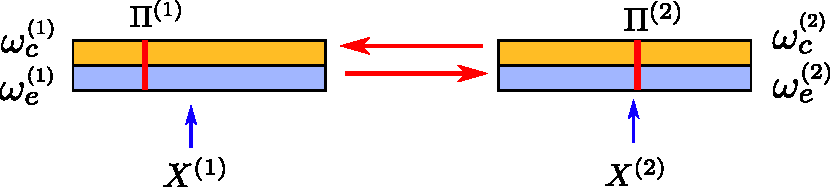
\includegraphics[width=0.6\textwidth]{archi_2som}
\caption{Architecture la plus simple possible de deux cartes. Le BMU $\bmu\m{1}$ de la carte $M\m{1}$ est utilisé en entrée de $M\m{2}$, et le BMU $\bmu\m{2}$ de $M\m{2}$ en entrée de $M\m{1}$. Chaque carte possède donc deux couches de poids. \label{fig:2som_archi}}
\end{figure}
\begin{figure}
\centering
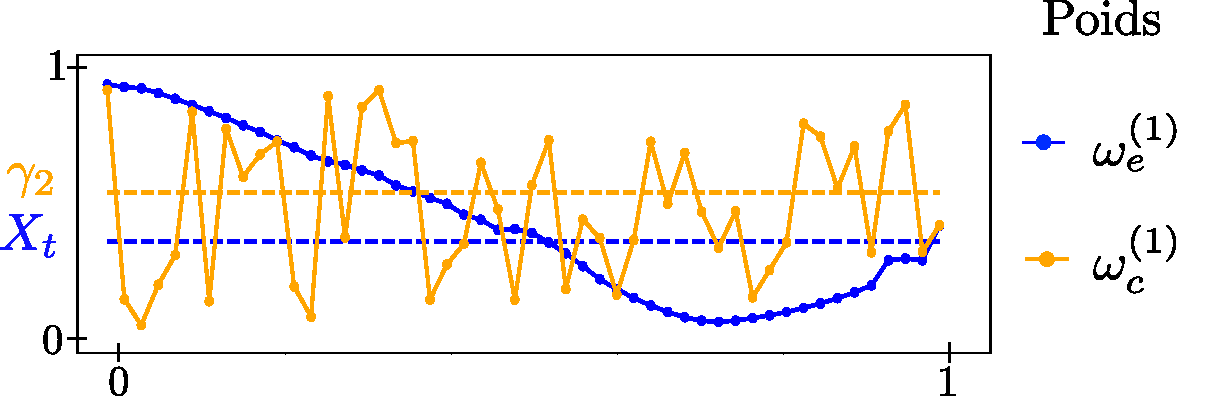
\includegraphics[width=0.75\textwidth]{weights_2som.pdf}
\caption{Représentation des poids de $M\m{1}$. L'entrée externe $\inpx_t$ présentée à l'itération $t$, tirée d'un espace d'entrée 1D $[0,1]$, est indiquée en bleu sur le graphique. L'entrée contextuelle  est $\inpc\m{1}$, le BMU de la carte $M\m{2}$. Sa valeur est indiquée en jaune; il s'agit d'une position 1D dans la carte $M\m{2}$, à valeur entre 0 et 1. L'exemple de disposition des poids est pris au cours du dépliement d'une structure de deux cartes sur un cercle. \label{fig:2som_weights}}
\end{figure}
\paragraph{Relaxation}
Le calcul de $\bmu\m{1}$ dépend donc de $\bmu\m{2}$ et inversement. Contrairement à une carte simple, on ne peut pas calculer tous les BMUs de l'architecture un par un en prenant $\hat{p}$, l'argmax de $a_g$, comme BMU dans chaque carte.
On remplace l'étape de simple calcul d'argmax par un processus global à l'architecture de recherche de BMU. Cette recherche est réalisée par un processus dynamique que l'on appelera \emph{relaxation}, menant à un consensus entre cartes : on cherche un point, s'il en existe, où le BMU de chaque carte est au plus proche du maximum de son activité globale $\hat{p}$. On répétera donc le calcul de l'activité globale et de son argmax plusieurs fois au sein d'une même itération.
Cette recherche est une boucle imbriquée dans un pas d'apprentissage $t$, indexée par $\tau$ et appelée relaxation. On définit une suite de BMUs intermédaires, $(\bmu\m{1}_\tau , \bmu\m{2}_\tau)$, $\tau$ variant de $0$ à un nombre d'itération maximum fixé pour assurer une fin de la boucle. Le processus de relaxation est le suivant:
\begin{enumerate}
\item Les entrées externes sont présentées au début de la boucle, donc $a_e$ peut être calculée; $\bmu\m{1}_0$ et $\bmu\m{2}_0$ sont initialisées à la position où les activités externes sont maximales dans chaque carte. 
\item On effectue des petits déplacements de $\bmu\m{1}$ et $\bmu\m{2}$ dans chaque carte. Tant que la suite de positions $(\bmu\m{1}_\tau,\bmu\m{2}_\tau)$ n'a pas atteint un point de convergence:
	\begin{enumerate}
	\item Dans chaque carte, calculer les activités contextuelles et globales, définissant ainsi $\hat{p}\m{1}_\tau = \argmax_{p\m{1}}(a_g\m{1}(p\m{1},\inpx\m{1}, \bmu\m{2})$, de même pour $\hat{p}\m{2}$.
	\item Déplacer $\bmu\m{1}$ vers $\hat{p}\m{1}$ et $\bmu\m{2}$ vers $\hat{p}\m{2}$ d'un pas $\Delta$: $\bmu\m{1}_{\tau+1} = \bmu\m{1}_{\tau} \pm \Delta$.
	Si une des valeurs est plus proche de $\hat{p}$ que $\Delta$, on déplacera $\bmu$ directement sur $\hat{p}$ pour éviter les oscillations autour du point. Cette étape est illustrée en figure~\ref{fig:relax}.
	\end{enumerate}
\item Le BMU de chaque carte est pris comme la valeur finale stable de ce processus dynamique. On note cette position finale $\bmu\m{i}_t$, désignant que cette valeur correspond à l'itération d'apprentissage $t$. Cette valeur est utilisée pour les mise a jour des poids. Si la relaxation n'atteint pas de point stable, on fixe tout de même un nombre d'itérations maximum après lequel on arrête la relaxation.
\end{enumerate}
\paragraph{Mise à jour}
Enfin, chaque couche de poids $\w\ext\m{i}$, $\w_c\m{i}$ est mise à jour indépendamment dans chaque carte relativement au BMU $\bmu\m{i}_t$ et les entrées externes $\inpx\m{i}_t$ et contextuelles $\bmu\m{j}_t$. Cette mise à jour correspond à la figure~\ref{fig:maj}. Les rayons d'apprentissage sont différents entre couche externe et couche contextuelle.

\begin{figure}
\centering
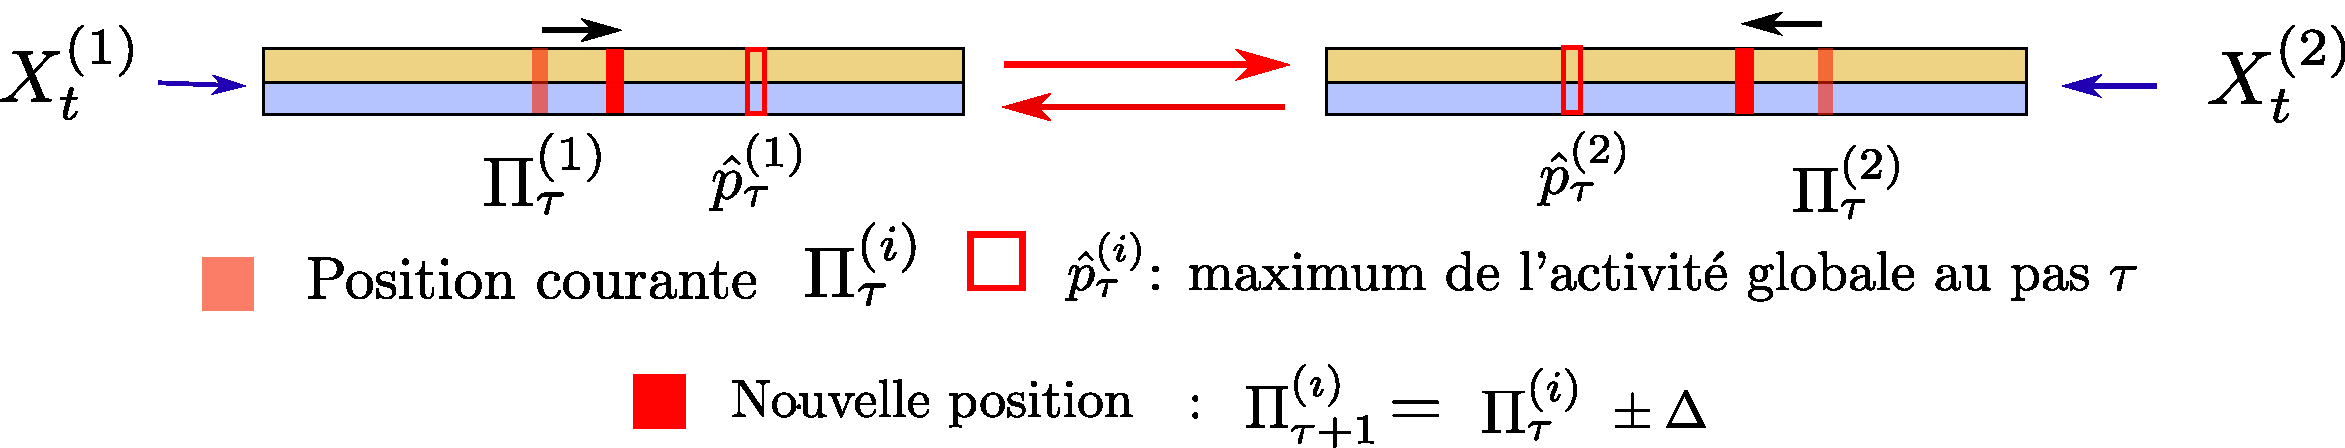
\includegraphics[width=\textwidth]{relaxation_2maps.pdf}
\caption{description d'une étape de la relaxation dans l'architecture, aboutissant à un consensus entre cartes. Au sein d'une même itération $t$, les position des BMU $\bmu$ sont légèrement déplacées jusqu'à ce que toutes les positions $\bmu$ des cartes de l'architecture soient stable. Ces positions maximisent collectivement les activités globales de chaque carte. \label{fig:relax}}
\end{figure}

\begin{figure}
\begin{minipage}{0.6\textwidth}
\centering
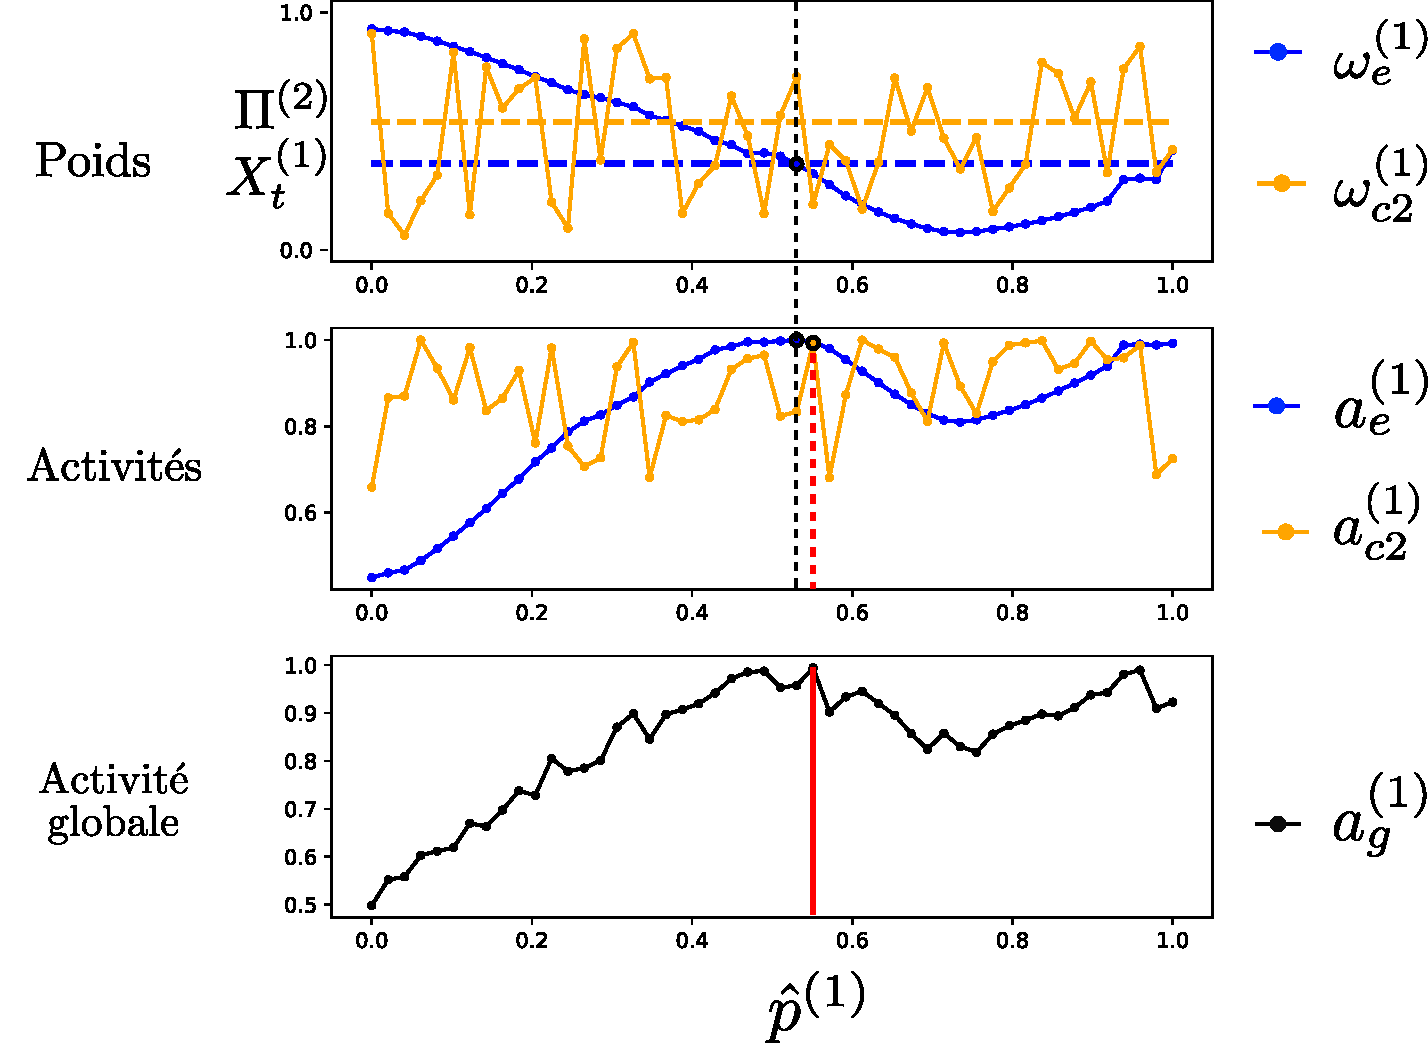
\includegraphics[width=\textwidth]{activite_layers_2maps.pdf}
\end{minipage}
\hfill
\begin{minipage}{0.35\textwidth}
\caption{Calcul d'activité dans une SOM au sein d'une architecture de deux cartes. La carte prend une entrée externe et une entrées contextuelle. L'indice $(1)$ permet de distinguer les objets relatif à cette carte. L'entrée externe est $X\m{1}_t$. La carte possède deux couches de poids, permettant de calculer deux activités. L'activité globale prend en compte tout les couches d'activités afin de trouver un BMU commun pour toutes les couches de poids. Ce calcul favorise l'activité externe et est modulé par l' activité contextuelle, ce qu'on observe sur la courbe du bas. Le maximum de l'activité globale est noté $\hat{p}$. A partir de l'activité globale, le BMU $\bmu\m{1}$ sera trouvé par le processus de relaxation décrit en partie~\ref{sec:relax}\label{fig:2som_activite}}
\end{minipage}

\end{figure}

\begin{figure}
\begin{minipage}[c]{0.6\textwidth}
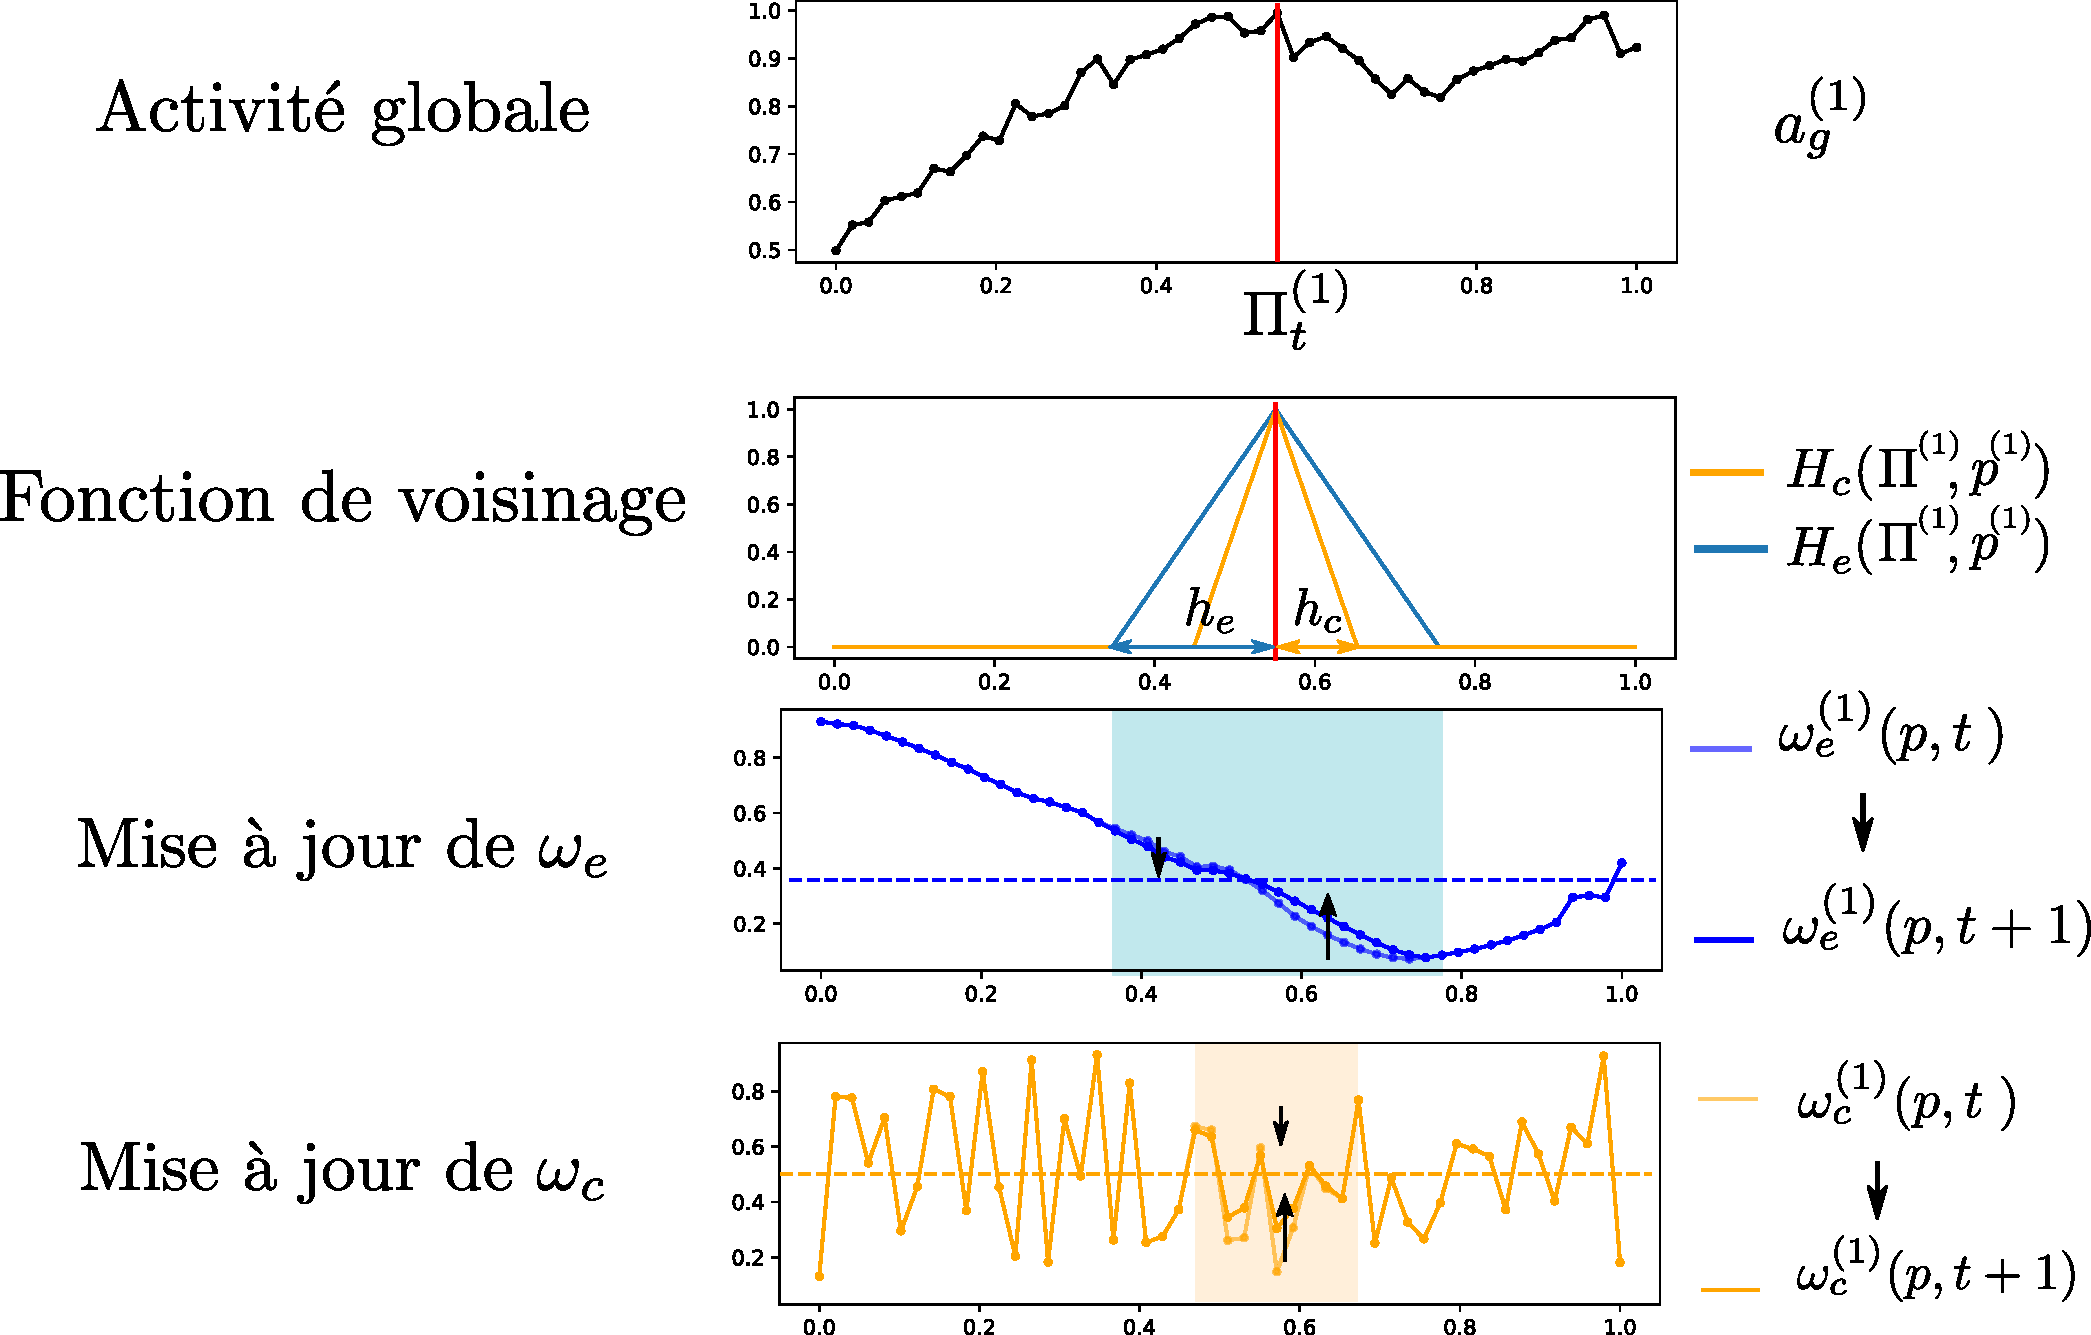
\includegraphics[width=\textwidth]{maj_2som.pdf}
\end{minipage}
\hfill
\begin{minipage}[c]{0.35\textwidth}
\caption{Mise à jour de chaque couche de poids indépendamment, relativement au BMU commun $\bmu\m{1}$, calculé par relaxation. Par définition de la relaxation, la position $\bmu\m{1}$ est proche de la position $\hat{p}\m{1}$ à la fin de la relaxation. Le rayon de voisinage $h_e$ est utilisé pour mettre à jour les poids externes, le rayon $h_c$ pour mettre à jour les poids contextuels. On choisit $h_e > h_c$. Cette différence permet une différence d'échelle d'apprentissage entre couches de poids. Elle est détaillée en section suivante.\label{fig:maj}}
\end{minipage}
\end{figure}

\subsection{Résumé}
Les étapes d'un pas d'apprentissage $t$ d'une architecture de deux cartes sont les suivantes; elles sont schématisées en figure~\ref{fig:algo}.
\begin{enumerate}
\item Présentation des entrées $\inpx\m{1}_t$ et $\inpx\m{2}_t$ à chaque carte
\item Relaxation:
\begin{enumerate}
\item Calcul de l'activité externe $a_e(\inpx\m{i},p)$ dans chaque carte et initialisation des BMUs $(\bmu\m{1}_0,\bmu\m{2}_0)$ pour la relaxation.
\item Relaxation par petits déplacements de $\bmu\m{1}_\tau,\bmu\m{2}_\tau$ dans chaque carte, avec calcul de l'activité contextuelle et globale à chaque pas $\tau$, jusqu'à stabilisation selon $\tau$ du couple de valeurs $(\bmu\m{1}_\tau,\bmu\m{2}_\tau)$
\item Choix des positions de BMU $\bmu\m{1}_t,\bmu\m{2}_t$ comme la valeur de $(\bmu\m{1}_\tau,\bmu\m{2}_\tau)$ à l'issue de la relaxation
\end{enumerate}
\item Mise à jour des poids $\w\ext\m{i}$ et $\w\cont\m{i}$ dans chaque carte, selon la position du BMU $\bmu\m{i}$, les entrées externes $\inpx\m{i}_t$ et contextuelles $\bmu\m{j}_t$, la position du BMU calculée par relaxation dans l'autre carte.
\end{enumerate}

\begin{figure}
\centering
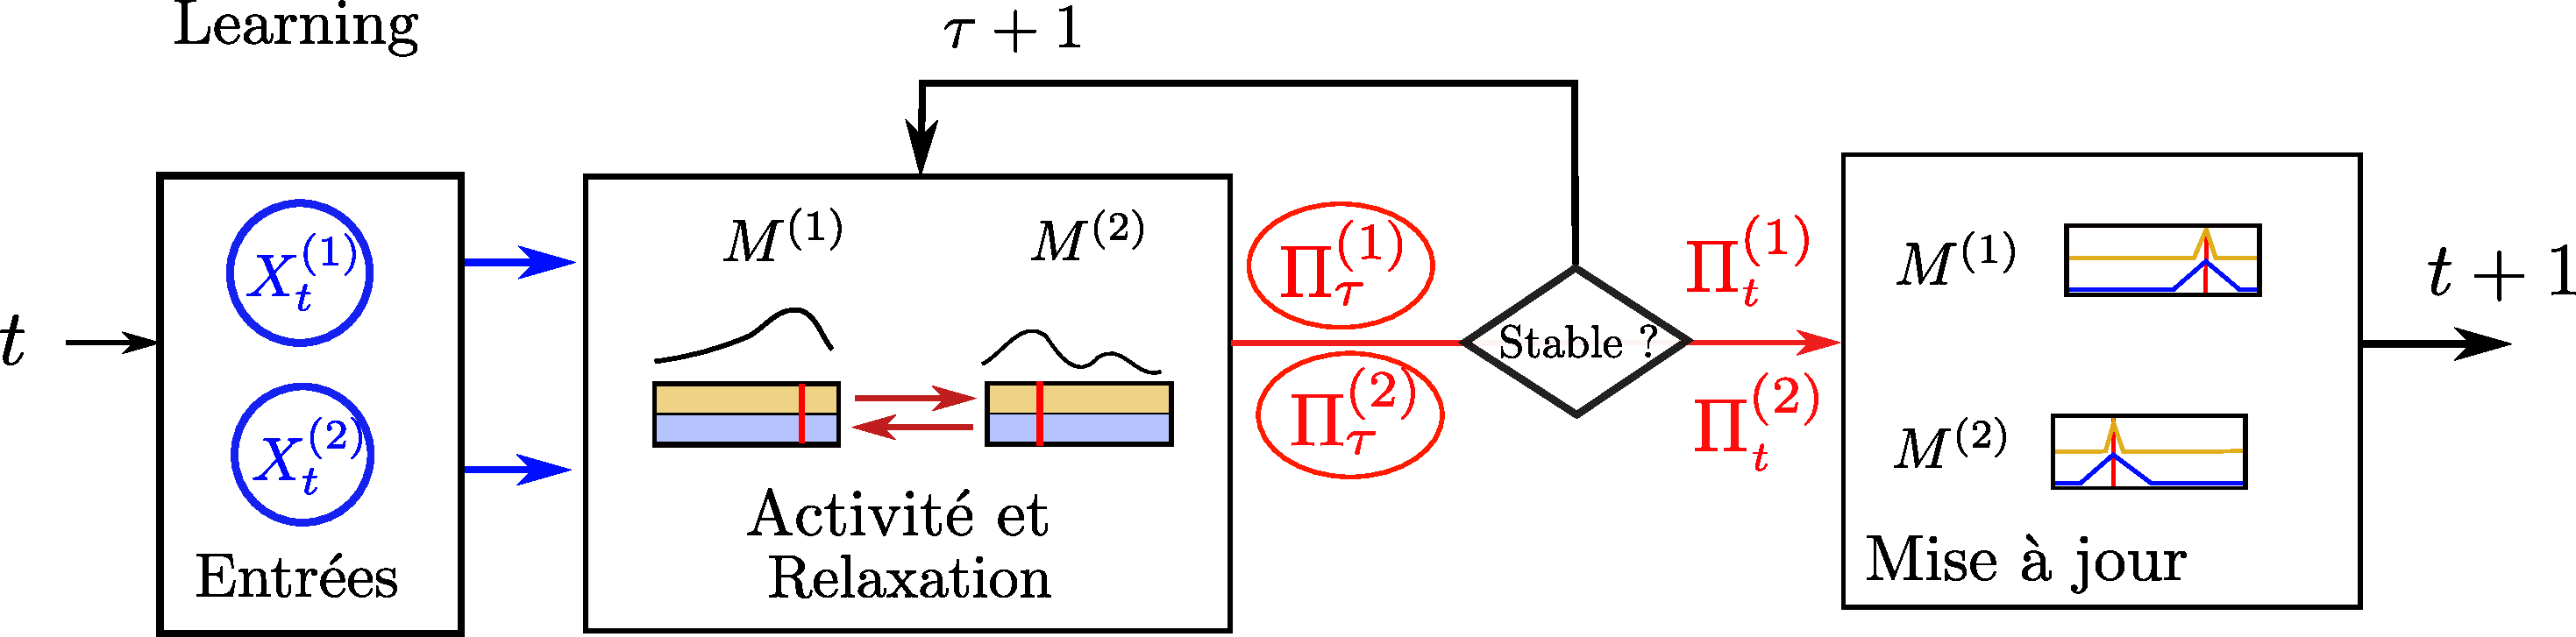
\includegraphics[width=\textwidth]{learning_tests_2maps}
\caption{Résumé des étapes de l'algorithme d'apprentissage d'une architecture.}
\label{fig:algo}
\end{figure}





\section{Formalisation: cas pour $n$ cartes}\label{sec:formalisme}

Nous présentons dans cette partie un formalisme pour l'algorithme général pour une architecture quelconque de $n$ cartes. Les notations sont valables pour des cartes de dimension quelconque; les entrées peuvent être de dimension quelconque.
La différence principale avec l'exemple à deux cartes est qu'une carte peut prendre plusieurs entrées contextuelles, qui sont les BMUs de toutes les cartes qui lui sont connectées dans l'architecture, au lieu d'une dans le cas de deux cartes. On retrouvera donc les notations de la partie précédente.
Cette partie concentre toutes les notations et l'algorithme utilisé dans cette thèse. L'algorithme est résumé en algorithme~\ref{algo:cxsom}.

\subsection{Entrées et calcul d'activité}
Nous présentons d'abord la structure et les notations utilisées dans une carte; toutes ces notations sont retrouvables en figure~\ref{fig:2som_activite}, pour l'exemple d'architecture de 2 cartes. Dans une architecture composée de $n$ cartes, les cartes sont indexées par $i \in \{1,\cdots,n\}$. On indicera chaque élément d'une carte $M\m{i}$ par l'exposant $(i)$.
Pour faciliter la lecture, nous omettrons par abus de langage l'exposant $(i)$ dans les équations, lorsqu'on se concentre sur une seule carte. $\inpx_t$ désigne donc $\inpx_t\m{i}$, $\w_e$ désigne $\w_e\m{i}$, etc.


A un pas d'apprentissage $t$, une carte $M\m{i}$ reçoit en entrée une entrée \emph{externe} notée $\inpx_t$ et $K$ entrées \emph{contextuelles}. Notons les pour le moment $\inpc_{i_1},\cdots,\inpc_{i_K}$; elles seront les positions de BMU $\bmu\m{i_k}$ des cartes d'indice $i_k$ qui lui sont connectées. La gestion des entrées contextuelles sera décrite avec le processus de relaxation en section suivante; notons pour le moment que les entrées contextuelles sont des positions 1D ou 2D dans des cartes. 

La carte possède donc $K+1$ couches de poids. On  note $\w_e(p)$ les poids externes et $\w_{ci_1}(p), \cdots, \w_{ci_K}(p)$ les poids correspondant aux entrées contextuelles, les \emph{poids contextuels}. Les poids externes sont à valeur dans $\mathcal{D}\m{i}$, la modalité associée à la carte $i$. Les poids contextuels sont à valeur dans l'espace des positions d'une cartes, soit $[0,1]$ en 1D ou $[0,1]^2$ en 2D.

Les activités externes et contextuelles s'expriment de la façon suivante:
\begin{equation}
\label{eq:activite}
\begin{cases}
a_e(\inpx_t,p) = \exp\frac{-\lVert \w_e(p)-\inpx_t \rVert^2}{2\sigma^2} \\
a_{ci_k}(\inpc_{i_k},p) = \exp\frac{-\lVert \w_{ci_k}(p)-\inpc_{i_k} \rVert ^2}{2\sigma^2}, \\
i_1, \cdots, i_K\: \text{indices des cartes connectées à $i$ dans l'architecture}
\end{cases}
\end{equation}
Notons $a_c(\Gamma,p)$ la moyenne des activités contextuelles, avec $\Gamma = (\inpc_{i_1}, \cdots, \inpc{i_K})$.
\begin{equation}
a_c(\Gamma,p) = \frac{1}{K}\sum_{k=1}^K {a_{ci_k}(\inpc_{i_k},p)}
\end{equation}
L'activité globale $a_g$ est calculée en combinant l'activité externe et la moyenne des activités contextuelles:
\begin{equation}
\label{eq:global_act}
a_g(\inpx_t,\Gamma,p) = \sqrt{a_e(\inpx_t,p)(\beta a_e(\inpx_t,p) + (1-\beta) a_c(\Gamma,p)}, \; \beta=0.5
\end{equation} 
On note $\hat{p}$ la position du maximum de l'activité globale:
\begin{equation}
\label{argmax}
\hat{p} = \argmax_p a_g(\inpx_t, \Gamma,p)
\end{equation}

\subsection{Calcul du BMU par relaxation}\label{sec:relax}

\paragraph{Formulation du problème de recherche de BMU}
Dans chaque carte $i$, l'entrée contextuelle $\inpc\m{i}_{i_k}$ est le BMU $\bmu\m{i_k}$  de la carte $i_k$. Le BMU $\bmu\m{i}$ dépend donc de ceux des autres cartes, qui dépendent eux-mêmes de $\bmu_m{i}$. Au lieu de chercher un maximum d'activité indépendamment dans chaque carte, on doit donc résoudre un problème d'optimisation global à  l'architecture. On cherche les positions $\mathbf{\bmu} = (\bmu\m{1}, \cdots, \bmu\m{n})$, si elles existent, telles que:
\begin{equation}
\forall i, \; \bmu\m{i} = \argmax_{p\m{i}} a_g\m{i}(\inpx\m{i}_t, \bmu\m{i_1}, \cdots, \bmu\m{i_K},p\m{i})
\end{equation}
$\bmu\m{i_1}, \cdots, \bmu\m{i_K}$ est un sous ensemble de $\mathbf{\bmu}$. On peut donc écrire $\bmu\m{i} = \argmax_{p\m{i}} a_g\m{i}(\inpx\m{i}_t, \mathbf{\bmu}, p\m{i})$
Si cette position n'existe pas, on cherche le meilleur compromis, c'est à dire les positions $\bmu\m{i}$ telles que l'activité globale de chaque carte soit la plus élevée possible.


Pour formuler le problème en terme d'optimisation, on cherche le vecteur $\mathbf{\bmu} = (\bmu\m{i})_{i=1 \cdots n}$ minimisant, pour tout $i$, $\lVert \bmu\m{i} - \argmax_{p\m{i}} a_g\m{i}(\inpx\m{i}_t, \mathbf{\bmu}, p\m{i}) \rVert$

\paragraph{Heuristique de recherche de BMU}
Le processus de relaxation est une boucle imbriquée dans un pas d'apprentissage de l'architecture, indexée par $\tau$. Notons $\bmu\m{i}$ la position du BMU de la carte $i$, et $\mathbf{\bmu} = (\bmu\m{0}, \cdots , \bmu\m{n})$, avec $n$ le nombre de cartes de l'architecture.

On cherche, dans chaque carte $i$, la position $\bmu\m{i}$ telle que $\forall i, a_g\m{i}(\bmu\m{i},\inpx\m{i},\bmu\m{i_0},\cdots,\bmu\m{i_k})$ soit maximale.
Au début d'un pas d'apprentissage, chaque carte est nourrie avec une entrée externe $\inpx\m{i}_t$ qui restera constante au cours de la relaxation. Les activités externes $a_e\m{i}(\inpx\m{i}_t,p)$ de chaque carte peuvent être calculées.
La recherche du BMU suit le processus de relaxation suivant :
\begin{enumerate}
\item Dans chaque carte $i$, la position $\bmu\m{i}$ est initialisée à $\hat{p}\m{i}_0 = \argmax_{p\m{i}}(a_e\m{i}(\inpx\m{i}_t,p)$. Dans chaque carte $i$, on assigne $\inpc_{i_k}\m{i} = \bmu\m{i_k}_\tau$
\item Tant que toutes les positions $\bmu\m{i}$ ne sont pas stables, 
	\begin{enumerate}
	\item Dans chaque carte $i$, calculer les activités contextuelles et globales, définissant ainsi $\hat{p}\m{i}_\tau = \argmax_{p\m{i}}(a_g\m{i}(p\m{i},\inpx\m{i}, \bmu\m{i_0}_\tau,\cdots,\bmu\m{i_k},_\tau)$, avec $i_0, \cdots, i_k$ les indices des cartes connectées à $i$ dans l'architecture.
	\item Déplacer $\bmu\m{i}$ vers $\hat{p}\m{i}$ : $\bmu\m{i}_{\tau +1} \leftarrow \bmu\m{i}_\tau \pm \Delta$ si $\lvert \bmu\m{i}- \hat{p}\m{i}\rvert \geq \Delta$, $\bmu\m{i} \leftarrow \hat{p}\m{i}$ sinon
	\end{enumerate}
\item Le BMU de chaque carte est pris comme la valeur finale stable de ce processus dynamique. Cette valeur est utilisée pour les mise a jour des poids.
\end{enumerate}

Il peut arriver que les positions ne trouvent pas de point de stabilité. Dans ce cas, on arrêtera la relaxation arbitrairement; ce phénomène étant ponctuel, il n'influence pas l'apprentissage. Les paramètres des cartes de l'architecture sont choisis pour éviter de telles situations.

\subsection{Mise à jour des poids}
Les poids sont mis à jour par rapport à leurs entrées respectives suivant l'équation \ref{eq:update}. Le BMU d'une carte est ainsi commun à toutes les couches. Les rayons de voisinage $h_e$ et $h_c$ ont des valeurs différentes ; celles-ci seront détaillée en partie suivante. 
Il faut noter que les poids contextuels cartographient l'espace des positions d'une autre carte. Les positions des cartes sont donc associées par les poids contextuels.
\begin{align}
 \w\ext\m{i}(p,t+1) = \w\ext\m{i}(p,t) + H\ext(\bmu\m{i}, p)(\w\ext\m{i}(p) - \inpx_t\m{i}) \\
\forall k, \w_{ck}\m{i}(p,t+1) = \w_{ck}\m{i}(p) + H\cont(\bmu\m{i},p)(\w_{ck}\m{i}(p) - \bmu\m{i_k}_t)
\end{align}

\begin{algorithm}\label{algo:cxsom}
\caption{Déroulement d'une itération d'apprentissage $t$}
\SetAlgoLined
  \KwData{$\inpx\m{1}_t, ... , \inpx\m{K}_t$ tirés dans $\mathcal{D}\m{1} \times \cdots \times \mathcal{D}\m{n}$}
  $\tau \leftarrow 0$ \;
  \lForEach{Carte $i$}{$\bmu\m{i}_0 \leftarrow \argmax_{p\m{i}} a\ext(\inpx\m{i}_t,p\m{i})$}
  \While {$\mathbf{\bmu}_\tau \neq \mathbf{ \bmu}_{\tau-1}$ et $\tau < N_{max}$}{
  \ForEach{Carte $i$}{
 	Avec $i_0, \cdots i_k$ indices des cartes connectées à $i$ dans l'architecture: \;
	Calcul de $a_{c1}\m{i}(\bmu\m{i_0},p\m{i}), \cdots, a_{ck}\m{i}(\bmu\m{i_k},p\m{i})$ \;
  	Calcul de $a_g\m{i}(\inpx\m{i}, \bmu\m{i_0}_\tau, \cdots, \bmu\m{i_k}_\tau)$ (equation~\ref{eq:global_act}) \;
  $\hat{p}\m{i}_\tau = \argmax_{p\m{i}} a_g\m{i}(\inpx\m{i}, \bmu\m{i_0}_\tau, \cdots, \bmu\m{i_k}_\tau)$ \;
  Déplacement de $\bmu\m{i}_\tau$ vers $\hat{p}\m{i}$ d'un pas $\Delta$:
  $\bmu\m{i}_{\tau+1} \leftarrow \bmu\m{i}_\tau + min(\Delta, \lvert \hat{p}\m{i} - \bmu\m{i} \rvert) \times \sign(\hat{p}\m{i} - \bmu\m{i})$ \;
  }
  $\tau \leftarrow \tau + 1$ \;
  }
  $\bmu\m{1}_t, \cdots, \bmu\m{n}_t \leftarrow \hat{p}\m{1}_\tau, \cdots , \hat{p}\m{n}_\tau$ \;
  \ForEach{Carte $i$}{
  $\w\ext\m{i}(p) \leftarrow \w\ext\m{i}(p) + H\ext(\bmu\m{i}, p)(\w\ext\m{i}(p) - \inpx_t\m{i})$ \;
  \lForEach{$k$}{$\w_{ck}\m{i}(p) \leftarrow \w_{ck}\m{i}(p) + H\cont(\bmu\m{i},p)(\w_{ck}\m{i}(p) - \bmu\m{i_k}_t)$}
  }
 \end{algorithm}


\subsection{Etape de test}

Afin d'étudier le dépliement des cartes, on effectue des itérations de \emph{test} pendant l'apprentissage. Ces étapes consistent à effectuer les étapes de présentation d'entrée, calcul d'activité et recherche du BMU par relaxation, mais pas l'étape de mise à jour des poids. Les poids des cartes restent donc figés pendant un ensemble de tests. Les entrées des cartes sont alors les entrées externes $\inpx\m{i}$ de test et les sorties sont les BMUs $\bmu\m{i}$ des cartes de l'architecture. 
Les entrées $\inpx\m{i}$ sont tirées du même espace que les entrées utilisées pendant l'apprentissage.

\subsection{Prédiction d'entrée}
Par construction, une carte de l'architecture CxSOM peut ne pas avoir d'entrée externe. Les activités considérées pour la recherche du BMU seront alors les activités contextuelles. On peut ainsi utiliser CxSOM pour des tâches de prédiction. Les données présentée à l'architecture sont $\inpx\m{1}, \cdots, \inpx\m{n}$, $n$ modalités. Ces modalités portent de l'information les unes sur les autres. 
L'architecture de cartes peut être vue comme un système dynamique réagissant à des données d'entrées.

\section{Choix des paramètres}\label{sec:params}

Le modèle CxSOM introduit des paramètres supplémentaires par rapport à une carte classiques. Nous présentons dans cette section les paramètres choisis. Les plages de valeur utilisées pour tous les paramètres d'une architecture sont résumées en tableau~\ref{tab:params}
\subsection{Paramètrage d'une carte}
On retrouve les mêmes paramètres dans CxSOM que sur une carte classique: taille de la carte, topologie et dimensions. 
Contrairement à une carte simple, on a maintenant un jeu de paramètre d'apprentissage par couche de poids d'une carte : pour chaque couche de poids $\w_e$ et $\w_{ck}$, on peut faire varier le taux d'apprentissage $\alpha$ et le rayon de voisinage $h_e$ ou $h_{ck}$.
On choisit de prendre un taux d'apprentissage $\alpha$ commun à toutes les couches dans un souci de simplicité. $\alpha$ restera constant au cours de l'apprentissage, contrairement à une carte classique dans laquelle $\alpha$ décroît.
On choisit de prendre une valeur $h_{ck} = h_c$ commune à toutes les couches de poids contextuels d'une carte. Ainsi, on apporte une symétrie dans les connexions: les carte réagissent de la même façon aux autres cartes.
On choisit par contre de prendre le rayon externe $h_e$ très supérieur au rayon contextuel. Nous prendrons au moins $h_e = 10 h_c$. Ce choix de paramètres apporte deux échelles de vitesse dans l'apprentissage, sans avoir à modifier les paramètres au cours du dépliement. Les poids externes se déplient alors très rapidement sur les données, quand les poids contextuels se déplacent très peu au début. Lorsque les poids externes sont organisés, l'apprentissage n'influence plus que les poids contextuels et ces derniers se déplient. Nous analyserons plus en détail l'apprentissage des cartes dans le chapitre suivant.

\subsection{Paramètres de l'architecture}
Certains paramètres sont relatifs à l'architecture. Il s'agit d'abord de $\Delta$, le pas d'apprentissage. Nous avons pris la même valeur de pas pour toutes les cartes. Cette valeur sera en général d'ordre $0.1$, c'est à dire un déplacement de $10\%$ de la taille de la carte, dans les expériences présentées dans les chapitres suivants. Nous verrons que la valeur de ce paramètre a finalement peu d'influence sur la relaxation; il faut juste veiller à ne pas le prendre trop petit, pour ne pas augmenter les temps de relaxation nécessaires. Le deuxième paramètre relatif à la relaxation est $N_{max}$, nombre maximum de pas de relaxation. Il sera fixé à 200 dans la plupart de nos expériences; nous verrons que la relaxation, si elle converge, le fait en une dizaine de pas.
Les connexions entre cartes sont prédéfinies et fixes. On choisit donc au préalable une taille d'architecture et un modèle. 

\begin{table}
\caption{Tableau récapitulatif des paramètres ayant une influence sur le comportement de l'algorithme CxSOM. Tous les paramètres relatif à une carte sont les mêmes pour chacune des cartes de l'architecture, mais il est possible de les différencier. L'analyse de l'influence des paramètres sera détaillée au chapitre~\ref{chap:analyse}.}\label{tab:params}
\vspace{3mm}
\begin{tabular}{|c|c|c|}
\hline
Paramètres & Description & Plage de valeur \\
\hline
$\alpha$ & Taux d'apprentissage & $0.1$ \\
$N$ & Taille de la carte & de $500$ à $1000$ en 1D, $50 \times 50$ en 2D \\
$\h_e$ & Rayon de voisinage externe & autour de $0.2$ \\
$h_c$ & Rayon de voisinage contextuel & D'ordre $\frac{h_e}{10}$ ou inférieur) \\
$\Delta$ & Pas de relaxation & $0.1$ \\
\hline
\end{tabular}
\end{table}


\section{Conclusion}

le modèle CxSOM permet de construire une architectures de carte auto-organisatrices apprennant chacune sur des entrées de différent types, mais liées par un modèle: des entrées multimodales. L'apprentissage est couplé entre cartes par l'utilisation d'entrée contextuelles dans chaque carte, qui sont les positions des best matching unit des cartes qui lui sont connectées. Nous avons décrit dans ce chapitre l'algorithme permettant d'effectuer l'apprentissages de données dans une telle architecture ainsi que les notations associées.

L'algorithme d'apprentissage a été conçu de façon large: nous avons développé un modèle général permettant d'associer des cartes. Les objectifs des chapitres suivants sont d'abord de montrer le comportement de l'algorithme et comment la relaxation permet de déterminer un BMU dans chaque carte. Nous étudierons ensuite en détail comment les données fournies en entrées à une architecture sont représentées dans les couches de poids. Nous verrons enfin une application d'une architecture de cartes dans un contexte de prédiction d'entrée.

\draft{
\Annexes
\Annex{Glossaire des notations}
\begin{itemize}
\item $\inpx_t$ Entrée externe présentée à la carte à l'itération d'apprentissage $t$. $\inpx_t \in \mathcal{D}$
\item $\inpc$ Entrée contextuelle d'une carte. Les entrées contextuelles sont les positions des BMUs $\bmu\m{i_k}$ d'autres cartes de l'architecture; on notera $\inpc_{i_k}$ l'entrée contextuelle liée à la carte $i_k$.
\item $p$ indexation des noeuds carte, $p \in [0,1]$ ou $[0,1]^2$.
\item $\w\ext(p)$ Poids externes. $\w\ext \in \mathcal{D}$
\item $\w_{ck}(p)$ Couche de poids contextuels d'une carte liés à l'entrée $\inpc_{i_k}$. $\w_{ck}(p) \in [0,1]$ ou $[0,1]^2$.
\item $a_e(\inpx_t,p)$ Activité externe 
\item $a_{ck}(\inpc_{i_k},p)$ Activité contextuelle calculée sur la couche de poids $w_{ck}$
\item $a_c(\Gamma,p)$ Moyenne des couches activités contextuelles
\item $a_g(\inpx_t,\Gamma,p)$ Activité globale, combinaison des activités externes et contextuelles
\item $\bmu_\tau$ Positions intermédiaires des BMUs d'une carte pendant la relaxation
\item $\bmu_t$ Position finale du BMU d'une carte après relaxation
\end{itemize}
}
